\documentclass[12pt]{report}
%\usepackage[a4paper, total={15cm, 20cm}]{geometry}

\usepackage{amsmath}
\usepackage{amsthm}
\usepackage{amssymb}
\usepackage{graphicx}
\usepackage{natbib}
\usepackage{url}
\usepackage[nottoc]{tocbibind}

\DeclareMathOperator{\expfamily}{ExpFamily}
\DeclareMathOperator{\expectation}{E}
\DeclareMathOperator{\variance}{Var}
\DeclareMathOperator{\cov}{Cov}
\DeclareMathOperator{\corr}{Corr}
\DeclareMathOperator{\bernoulli}{Bernoulli}
\DeclareMathOperator{\betaDist}{Beta}
\DeclareMathOperator{\dirichlet}{Dir}
\DeclareMathOperator{\bin}{Bin}
\DeclareMathOperator{\MN}{Multinomial}
\DeclareMathOperator{\prob}{P}
\DeclareMathOperator{\trace}{Tr}

\newcommand{\RSS}{\mathrm{RSS}}
\newcommand{\euler}{\mathrm{e}}
\newcommand{\diff}{\mathrm{d}}
\newcommand{\T}{^\textup{T}}
\newcommand{\dotdotdot}{_{\phantom{.}\cdots}}

\newcommand{\vect}[1]{\mathbf{#1}}
\newcommand{\vectGreek}[1]{\boldsymbol{#1}}
\newcommand{\matr}[1]{\mathsf{#1}}

\newtheorem{theorem}{Theorem}
\newtheorem{algorithm}{Algorithm}


\begin{document}

%=====TITLE PAGE======
\begin{titlepage}
\centering
\vspace*{1cm}
        
        \LARGE
        \textbf{Inside-Out: Characterisation of Computed Tomography Noise in Projection and Image Space with Applications to 3D Printing}
        
		\large        
        
        \vspace{2cm}
        {OxWaSP 2015 Warwick Cohort - Mini-project 1}
        
        \vspace{1cm}
        {Sherman Ip}

        \vspace{1cm}
        {Supervisor: Dr.~J.~Brettschneider (Statistics, Warwick)}
        
        \vspace{1cm}
        {Supervisor: Prof.~T.~Nichols (Statistics, Warwick)}
        
        \vspace{1cm}
        {10th June 2016}
\end{titlepage}

%======ABSTRACT=========
\begin{abstract}
I did this. This happened. I should of done that.
\end{abstract}

%=====FRONT MATTER=====
\tableofcontents
%\listoffigures
%\listoftables

%======INTRODUCTION========
\chapter{Introduction}
Mini-project for OxWaSP.

%======LITERATURE REVIEW========
\chapter{Literature Review}
Computed tomography (CT) scanning is a 3D imaging technique. It does this by reconstructing the geometry of the sample through a series of 2D X-ray images of the sample. The sample rotates after each image taken.

Figure \ref{fig:x_ray_ct} shows a diagram on how CT scanning works. A 2D image is taken by projecting X-ray photons onto the stationary sample. The photons are then scattered or absobred by the sample.  Some of these photons are then detected by an X-ray detector on the other side of the sample, which produces an image. After an image has been taken, the object rotates and another image is taken. Finally after a number of images, a 3D reconstruction of the object can be estimated \cite{cantatore2011introduction}.

\begin{figure}
\centering
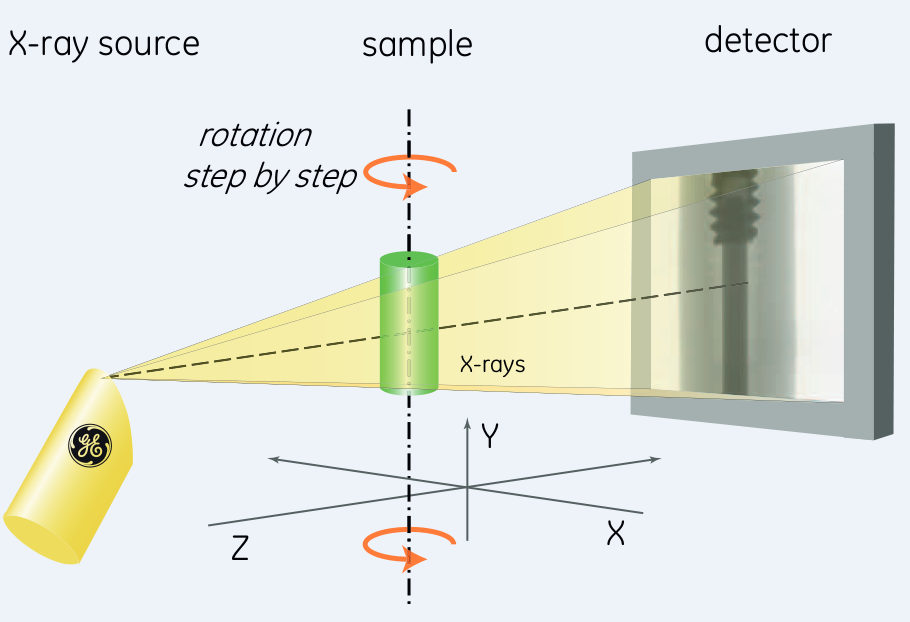
\includegraphics[width=0.7\textwidth]{figures/x_ray_ct.png}
\caption{X-ray computed tomography reconstructs the sample by firing X-ray photons onto a rotating sample. The photon are then detected by the detector. \emph{Source: http://www.phoenix-xray.com/}}
\label{fig:x_ray_ct}
\end{figure}

CT scanning was invented by G. Hounsfield \cite{hounsfield1980computed} in the 1980's and it was mainly used for medical imaging. The setup for CT scanning is different when scanning patients because the detector and X-ray source rotates around the patient \cite{cantatore2011introduction}. Recently CT has been used industrially for non-destructive testing in manufacturing \cite{cantatore2011introduction}. One possible application would be inspecting 3D printed (additive layer manufactured) samples.

There are many sources of error in CT scanning \cite{cantatore2011introduction} and this can cause problems when reconstructing the geometry of the sample. Sources of error include: defects in the detector, environmental noise and the behaviour of photons.

This chapter aims to give brief description on how CT scanning works and a short discussion on the sources of error.

\section{X-Ray Production}
X-ray photons in CT scanning are produced in an X-ray tube. In an X-ray tube, a cathode, consisting of a heated filament, fires projectile electrons through an electric potential to a target which forms the anode \cite{michael2001x}, as shown in Figure \ref{fig:x_ray_tube}. Most of the kinetic energy of the projectile electrons is converted into heat however some is converted into electromagnetic radiation. This depends on how the projectile electrons interact with the atoms in the anode \cite{cantatore2011introduction}.

\begin{figure}
\centering
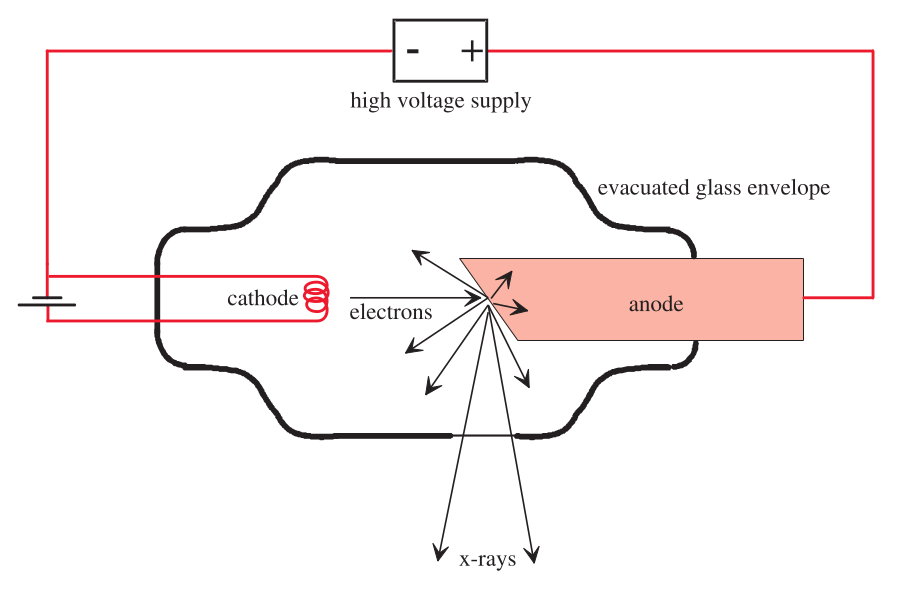
\includegraphics[width=0.8\textwidth]{figures/x_ray_tube.png}
\caption{An X-ray tube produces X-ray photons by firing projectile electrons from a cathode to an anode. \emph{Source: G.~Michael (2001) \cite{michael2001x}}}
\label{fig:x_ray_tube}
\end{figure}

Bremsstrahlung radiation is the result of projectile electrons deaccelerating due to the electrostatic field produced by nucleus of the target. The kinetic energy of the projectile electrons are then converted to electromagnetic radiation to produce X-ray photons. As a result, the photon energies in Bremsstrahlung is continuous spectrum and can range up to the maximum kinetic energy of the projectile electrons \cite{michael2001x}.

Characteristic radiation is due to projectile electrons colliding with electrons in the target atom and ionizing them. This produce vacancies in the electron shell and emits X-ray photons when the electrons in the target atom drops down back to the ground state. The energy of the emitted radiation is monoenergetic and depends on the binding energy of the target's atoms \cite{michael2001x}.

A typical energy spectrum of X-ray photons emitted from an X-ray tube is as shown in Figure \ref{fig:x_ray_spectrum}. The energy spectrum consist of both bremsstrahlung and characteristic radiation \cite{michael2001x}.

\begin{figure}
\centering
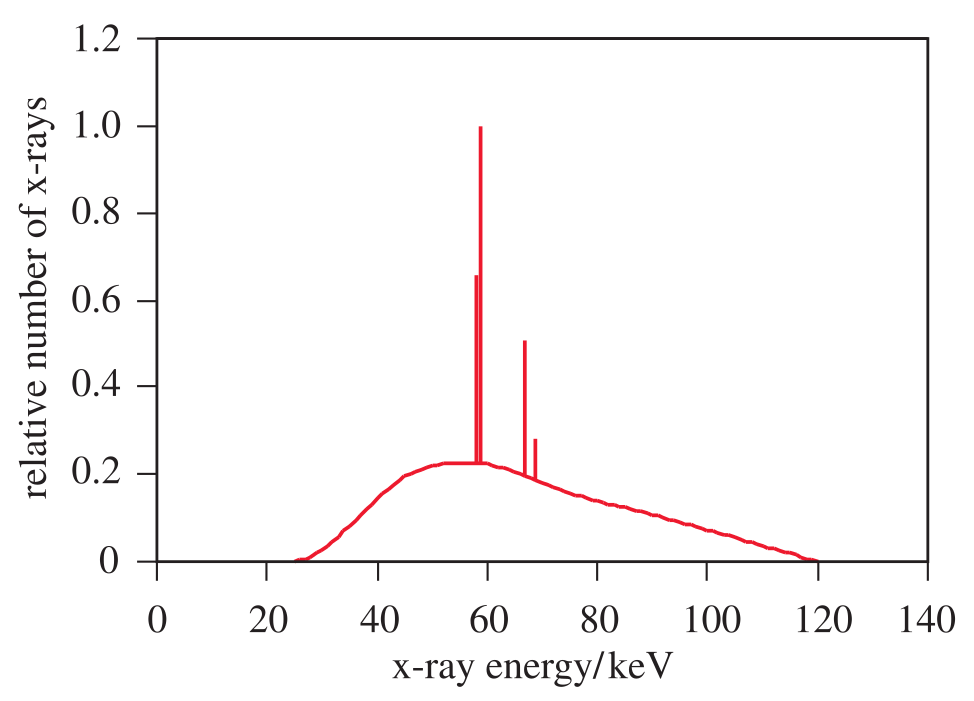
\includegraphics[width=0.8\textwidth]{figures/x_ray_spectrum.png}
\caption{A typical energy spectrum of X-ray photons emitted from an X-ray tube. The continuous spectrum is the result of Bremmsstrahlung radiation. The peaks are the result of characteristic radiation. \emph{Source: G.~Michael (2001) \cite{michael2001x}}}
\label{fig:x_ray_spectrum}
\end{figure}

The voltage, the energy per charge, and current, the rate of charge, can the varied in the X-ray tube to produce different energy spectrum and rate of X-ray emission. This can vary the results produced when collecting CT data \cite{cantatore2011introduction}. Another important factor is the focal spot size because smaller spot sizes produce sharper edges. Larger spot sizes produce unsharp results and this is know as the penumbra effect, as shown in Figure \ref{fig:x_ray_penumbra}. However spot sizes too small can produce concentrated heat \cite{welkenhuyzen2009industrial}.

\begin{figure}
\centering
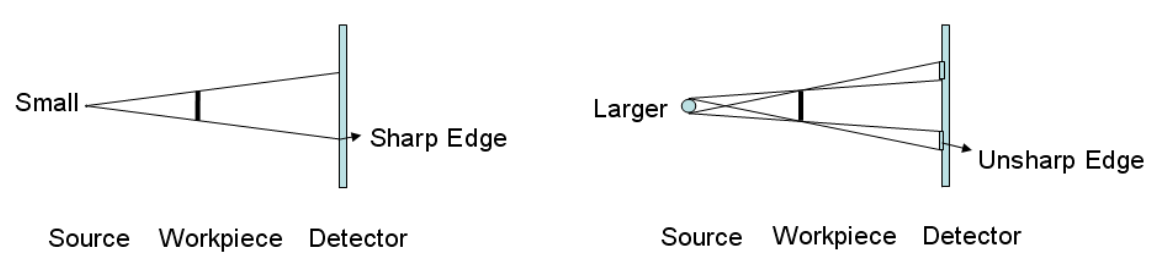
\includegraphics[width=1\textwidth]{figures/x_ray_penumbra.png}
\caption{Larger focal spot sizes produces unsharp results. This is know as the penumbra effect. \emph{Source: F.~Welkenhuyzen et al.~(2009)\cite{welkenhuyzen2009industrial}}}
\label{fig:x_ray_penumbra}
\end{figure}

\section{X-Ray Interactions}
X-ray photons emitted by the X-ray tube are fired onto the sample and interacts with it in a number of ways \cite{cantatore2011introduction}.

The sample can effectively absorb X-ray photons via the photoelectric effect or pair production \cite{cantatore2011introduction}. In the photoelectric effect, the X-ray photons transfers its energy to a bounded electron and ejects it from the atom \cite{millikan1916direct}. In pair production, the X-ray photons converts into an electron-position pair by interacting with the Coulomb field of the sample's atomic nucleus \cite{hubbell2006electron}.

X-ray photons can be scattered by the sample. This happens when X-ray photons collide inelastically with and transfers it's energy to the sample's electrons. This process is know as Compton scattering \cite{compton1923quantum}.

The attenuation (decrease in X-ray intensity from $I_0$ to $I_1$) when propagating though a material with attenuation coefficient $\mu$ and distance $x$ is given as
\begin{equation}
I_1 = I_0\euler^{-\mu x}
\end{equation}
where it was assumed the X-ray photons are monoenergetic \cite{michael2001x}. This can be extended to a continuous spectrum of X-ray energies by making $\mu$ dependent on the energy of the X-ray photons \cite{cantatore2011introduction}. In general low energy photons are more likely to be absorbed than high energy photons, this increases the average energy of the attenuated photons and can be a source of error in CT scanning. This is referred to beam hardening \cite{michael2001x}. This can be reduced by placing a thin sheet of filter to absorb low energy photons \cite{welkenhuyzen2009industrial} or by correcting it in the data analysis stage \cite{michael2001x}.

\section{Detector}
Most X-ray detectors are scintillator-photodiode detectors. The photons interact with the scintiallator material and produces visible light. The visible light is then detected by photodiodes and covert into electric current \cite{michael2001x}. The detectors used in CT scanning are flat bed scanner which consist of an array of panels of photodiodes \cite{cantatore2011introduction}.

\section{Reconstruction}
The scale of the 2D images are calibrated with the use of reference standards \cite{bartscher2007enhancement}. The method used to reconstruct the 3D geometry of the sample is called the filtered back-projection \cite{michael2001x}. The mathematics can be reviewed in \cite{brooks1976principles}.

\chapter{Exploratory Data Analysis}
\section{Summary Statistics}
\section{Principal Component Analysis}
\subsection{Theory}
\subsection{Methods}
\subsection{Results}
\section{Factor Analysis}
\subsection{Theory}
\subsection{Methods}
\subsection{Results}
\chapter{Mean and Variance Relationship}


\bibliographystyle{unsrt}
\bibliography{bib}
\end{document}